\clearpage
%%=========================================
\section{MCT Film Grown by MBE on  Substrate C}\label{sec:subCc}

A film of \acl{mct} was grown on substrate C by \ac{mbe}. Bright field microscopy images revealed that the surface of the \ac{mct} film was planar with a large number of angular features, as seen in Fig.~\ref{fig:subCc_om}.

\begin{figure}[htbp]
    \centering
    \mySubfigure{0.49\textwidth}{CMT801_om_bf_grid_14_10x.png}[fig:subCc_om_centre][angle=180]
    \hfill
    \mySubfigure{0.49\textwidth}{CMT801_om_bf_grid_21_10x.png}[fig:subCc_om_corner][angle=180]
    \caption[Bright field microscopy images of \ac{mct} film grown by \ac{mbe} on substrate C.]{Bright field microscopy images of \ac{mct} film grown by \ac{mbe} on (211)B-oriented substrate C: \subref{fig:subCc_om_centre} Near the centre; and \subref{fig:subCc_om_corner} near the lower left corner.}
    \label{fig:subCc_om}
\end{figure}

\citet{selvig2007defects} describe the irregularly shaped defects with sizes extending from \SI{10}{\micro\metre} to a few hundred microns as high temperature voids and the ones with size less than \SI{10}{\micro\metre} as microvoids. These types of defects are typically formed during the growth of the material and the density is dependent on the deviation from ideal growth conditions. High temperature voids are formed at substrate temperatures higher than the \ce{Te}-phase limit. Microvoids are formed at all substrate temperatures, but the density increases with lower substrate temperature. It was not observed any high temperature voids on the surface of the film, and hence, the film was grown at temperatures below the \ce{Te}-phase limit.

%\todo{Sammenlign med telling av tellurium precipitates->HT voids. Grit->microvoids.}

\begin{figure}[htbp]
    \centering
    \begin{subfigure}[t]{\textwidth}
        \caption{}\label{fig:subCc_microvoid}
          \begin{minipage}[c]{0.43\linewidth}
            \centering
            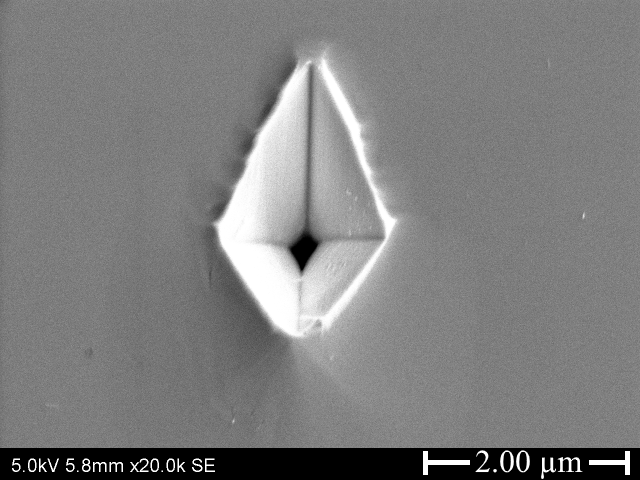
\includegraphics[width=\linewidth]{CMT801_sem_03_m002.png}
          \end{minipage}
          \hfill
          \begin{minipage}[c]{0.43\linewidth}
            \centering
            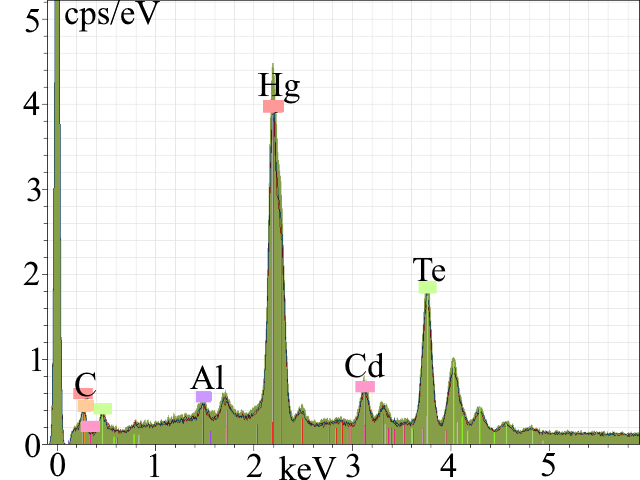
\includegraphics[width=\linewidth]{CMT801_sem_03_m002_eds.png}
          \end{minipage}
          \begin{minipage}[c]{0.11\linewidth}
            \centering
            \atomicTable[\ce{Te}&\SI{41.88}{}][\ce{Hg}&\SI{33.89}{}][\ce{C}&\SI{13.89}{}][\ce{Cd}&\SI{6.99}{}][\ce{Al}&\SI{3.35}{}]
          \end{minipage}
    \end{subfigure}
    \par\bigskip
    \begin{subfigure}[t]{\textwidth}
        \caption{}\label{fig:subCc_carbon_based}
          \begin{minipage}[c]{0.43\linewidth}
            \centering
            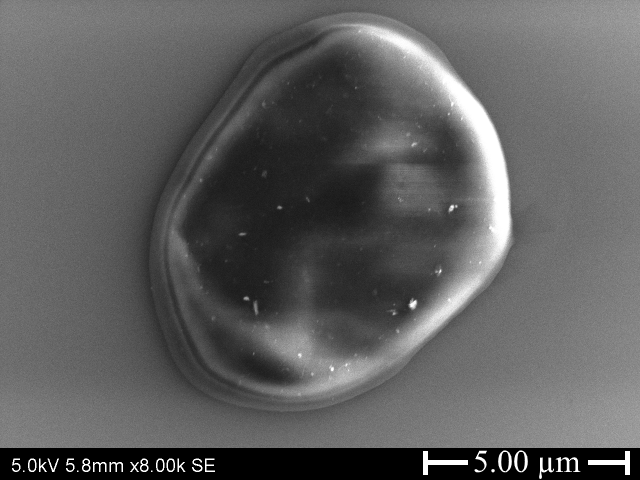
\includegraphics[width=\linewidth]{CMT801_sem_03_m006.png}
          \end{minipage}
          \hfill
          \begin{minipage}[c]{0.43\linewidth}
            \centering
            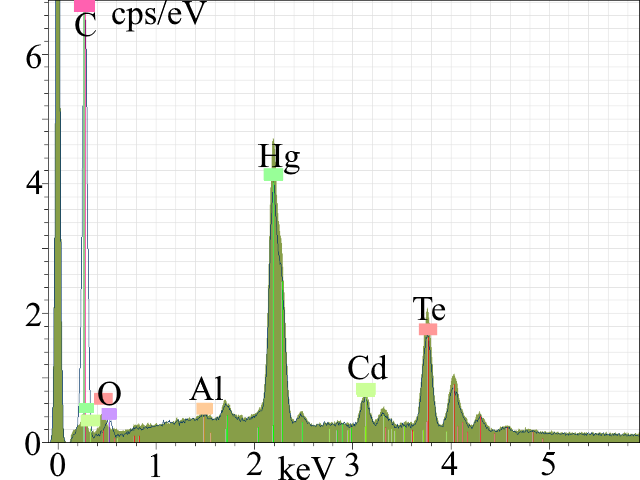
\includegraphics[width=\linewidth]{CMT801_sem_03_m006_eds.png}
          \end{minipage}
          \begin{minipage}[c]{0.11\linewidth}
            \centering
            \atomicTable[\ce{C}&\SI{77.12}{}][\ce{Te}&\SI{10.27}{}][\ce{Hg}&\SI{8.17}{}][\ce{O}&\SI{2.12}{}][\ce{Cd}&\SI{1.95}{}][\ce{Al}&\SI{0.37}{}]
          \end{minipage}
    \end{subfigure}
    \caption[\Ac{sem} images, \ac{eds} spectra, and \ac{eds} atomic compositions of one particle and one defect found on \ac{mct} film grown on substrate C.]{High-resolution \ac{sem} images of one defect and one particle found on the \ac{mct} film grown on substrate C and the corresponding \ac{eds} spectra and atomic compositions: \subref{fig:subCc_microvoid} Microvoid; and \subref{fig:subCc_carbon_based} carbon based particle. The blue line represents the \ac{eds} spectrum of the particle, while the filled green represents the \ac{eds} spectrum of the underlying substrate.}\label{fig:subCc_sem_w_eds}
\end{figure}

The size of the microvoids was between \SIrange{1}{3}{\micro\metre}. They were diamond-shaped with a longer axis towards the upper edge of the substrate and a shorter axis towards the right edge of the substrate, as seen in Fig.~\ref{fig:subCc_microvoid}. \Ac{eds} point spectra across the microvoids showed no difference between the composition of the microvoid and the surrounding layer. The microvoids were either single, single with some smaller microvoids around their edges, or in clusters, as seen in Fig.~\ref{fig:subCc_sem_microvoids}. The clusters typically consisted of \SIrange{3}{6}{} microvoids. % There was a hole in the centre of the diamond-shaped microvoid

\begin{figure}[htbp]
    \centering
    \mySubfigure{0.49\textwidth}{CMT801_sem_03_m001.png}[fig:CMT801_sem_03_m001]
    \hfill
    \mySubfigure{0.49\textwidth}{CMT801_sem_02_m013.png}[fig:CMT801_sem_02_m013]
    \caption[\Ac{sem} images of microvoids found in \ac{mct} film grown by \ac{mbe} on substrate C.]{\Ac{sem} images of microvoids found in \ac{mct} film grown by \ac{mbe} on substrate C: \subref{fig:CMT801_sem_03_m001} Cluster of diamond-shaped microvoids; and \subref{fig:CMT801_sem_02_m013} single diamond-shaped microvoids, some with smaller microvoids around their edges.}
    \label{fig:subCc_sem_microvoids}
\end{figure}

\begin{figure}[htbp]
    \centering
    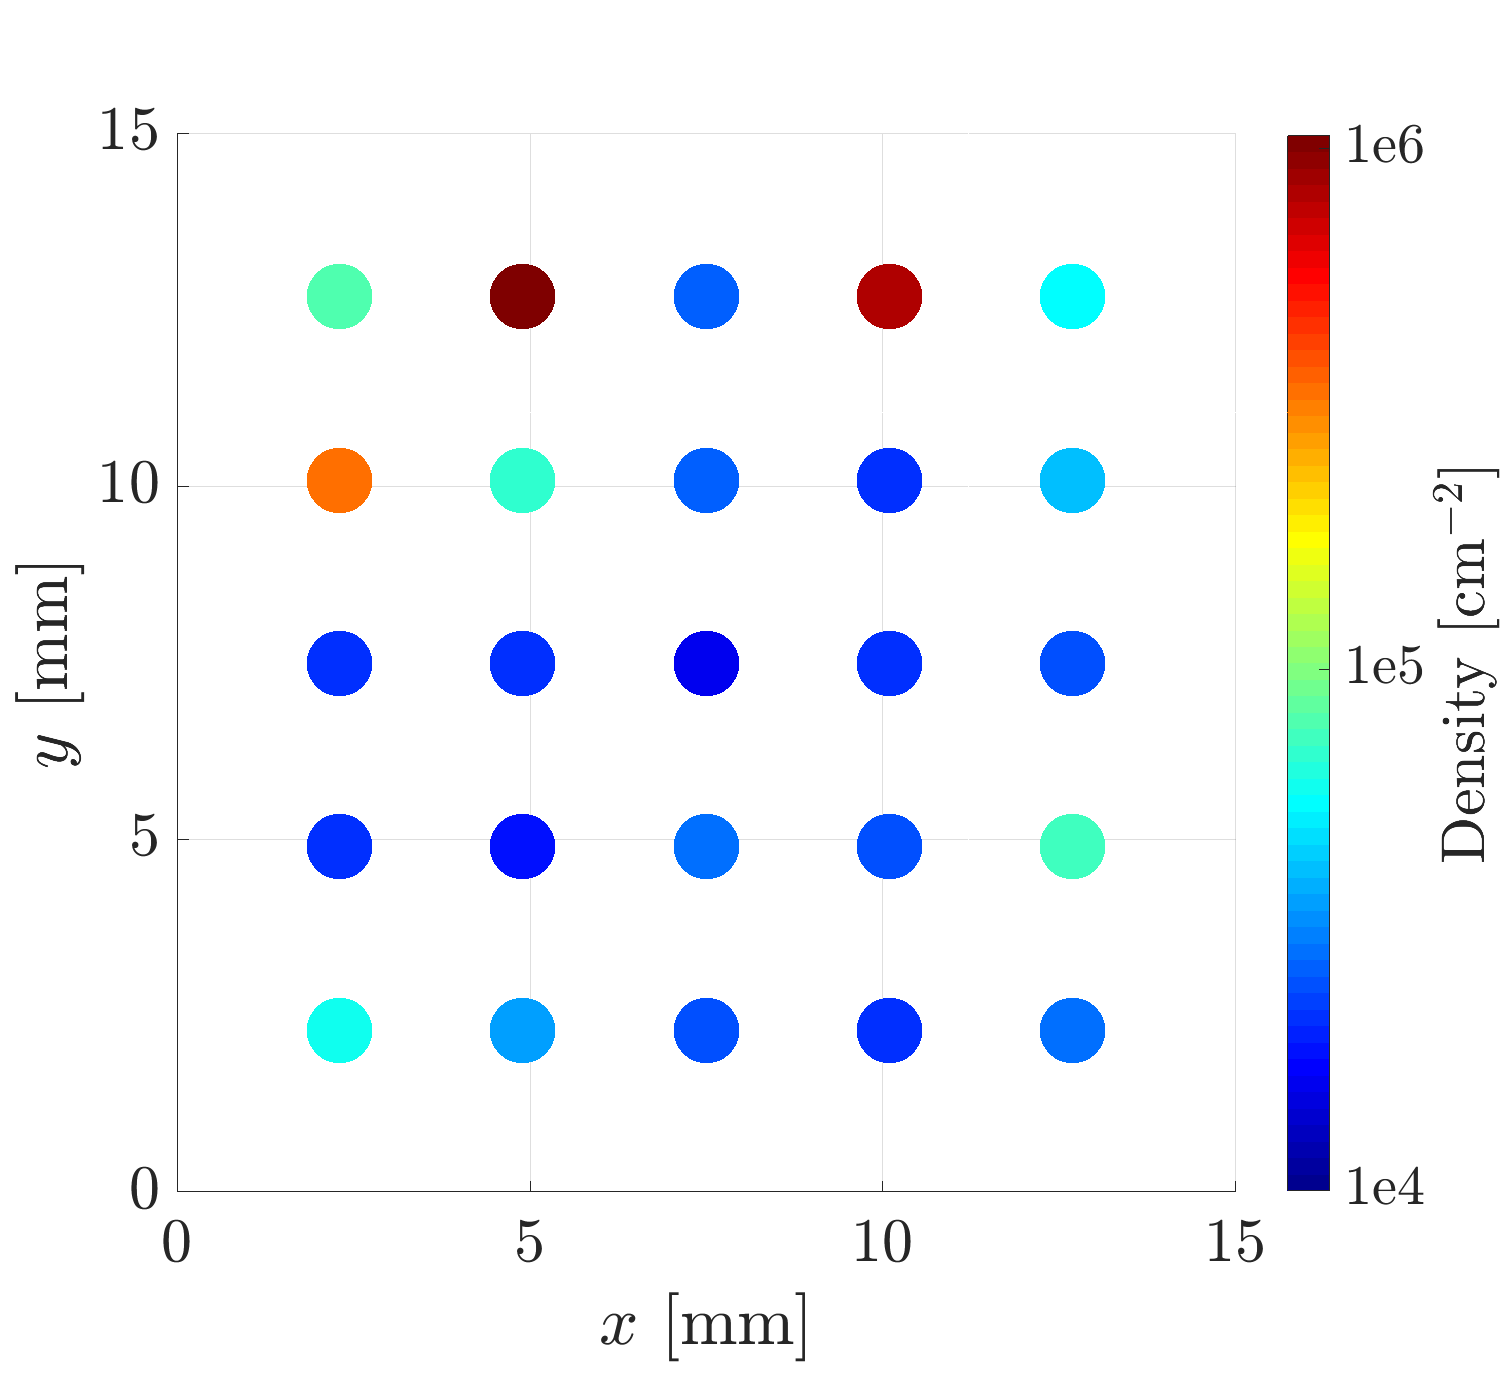
\includegraphics[width=0.5\linewidth]{CMT801_densityData.png}
    \caption[Map of the density of microvoids on the \ac{mct} film grown on substrate C.]{A map of the density of microvoids at 36 different locations on the $\SI{15}{\milli\metre}\times\SI{15}{\milli\metre}$ \ac{mct} film grown by \ac{mbe} on substrate C. The density measurements were obtained by counting the number of microvoids in bright field optical microscopy images covering $\SI{558}{\micro\metre}\times\SI{419}{\micro\metre}$ areas. In total, \SI{0.94}{\percent} of the substrate surface was measured. The density was observed to vary between \SIrange{2e+4}{1e+6}{\centi\metre^{-2}} with an average defect density of \SI{1e+05}{\centi\metre^{-2}}.}
    \label{fig:CMT801_densityData}
\end{figure}

The density of microvoids was found to be between \SIrange{2e+4}{1e+6}{\centi\metre^{-2}}. The average density was \SI{1e+05}{\centi\metre^{-2}} with a standard deviation of \SI{3e+05}{\centi\metre^{-2}}. The average density of the $3\times3$ centre points in the grid was \SI{3e+04}{\centi\metre^{-2}}, while the average density around the edges and corner was \SI{2e+05}{\centi\metre^{-2}}. A graphical representation of the density at different locations on the film can be seen in Fig.~\ref{fig:CMT801_densityData}. 

The sample Pearson correlation coefficient between the occurrence of polishing grit on the etched substrate C and the occurrence of microvoid defects on the film was determined to be \SI{0.40}{}, which is a moderate positive correlation. The residue from the evaporation of an acetone droplet, which settled on the surface while removing the etched substrate from the \ac{sem} holder, was clearly visible in the layer as a formation of microvoids, as seen in Fig.~\ref{fig:subCc_microvoids_correlation}. As the density of microvoids was counted from a larger area than the area used to count the density of polishing grit, this correlation coefficient is not entirely accurate and it could be even higher as the images in Fig.~\ref{fig:subCc_microvoids_correlation} indicate.

\begin{figure}[htbp]
    \centering
    \mySubfigure{0.49\linewidth}{subCb_om_df_n004_5x.png}[fig:subCb_om_df_n004_5x][angle=180]
    \hfill
    \mySubfigure{0.49\linewidth}{CMT801_om_bf_grid_04_10x.png}[fig:CMT801_om_bf_grid_04_10x][angle=180]
    \caption[Residue on etched substrate C visible as microvoids in the film.]{The residue from the evaporation of a acetone droplet on the etched substrate C was correlated with microvoids in the \ac{mct} film grown on substrate C: \subref{fig:subCb_om_df_n004_5x} Dark field microscopy image of etched substrate C; \subref{fig:CMT801_om_bf_grid_04_10x} bright field microscopy of \ac{mct} film.}\label{fig:subCc_microvoids_correlation}
\end{figure}

A second type of defect was observed on the film. This was a round particle with a size of \SIrange{4}{10}{\micro\metre}. The particle appeared darker than the substrate in \ac{sem} and did not have any sharp edges, as seen in Fig.~\ref{fig:subCc_carbon_based}. The \ac{eds} spectrum of the particle revealed that it mainly consisted of carbon. This type of particle was infrequent with respect to the microvoids with a density of \SI{\sim1e+02}{\centi\metre^{-2}}.

%%=========================================
\subsection{Composition and Thickness}

\Iac{ftir} transmission spectrum was recorded from one spot in the centre of the \ac{mct} film. The \ac{ir} transmittance was between \SIrange{50}{63}{\percent} in the wavenumber range between \SIrange{400}{1400}{\centi\metre^{-1}}, see Fig.~\ref{fig:subCc_ftir}. The cut-on wavenumber was \SI{1564.7}{\centi\metre^{-1}}, which corresponds to a wavelength of \SI{6.39}{\micro\metre}. Consequently, the $x$-value was \SI{0.224}{} according to the Brice equation \citep{brice1975some}. The thickness of the \ac{mct} film was calculated to be \SIrange{11.0}{11.6}{\micro\metre} by using Eq.~\ref{eq:ftir_thickness}.

%\todo{FTIR: correlate with polishing grit or donut density.}

\begin{figure}[htbp]
    \centering
    \mySubfigure{0.541578947\linewidth}{CMT801_ftir_spectra.png}[fig:subCc_ftir_spectra]%0.60175438596
    \hfill
    \mySubfigure{0.34042105262\linewidth}{CMT801_ftir_transmission_at_k500cm-1.png}[fig:subCc_ftir_map_500cm-1]%0.37824561403
    \caption[\Ac{ftir} measurement from one spot on the \ac{mct} film grown on substrate C.]{\Ac{ftir} measurements recorded from one spot on the $\SI{15}{\milli\metre}\times\SI{15}{\milli\metre}$ \ac{mct} film grown on substrate C: \subref{fig:subCc_ftir_spectra} Transmission spectrum; \subref{fig:subCc_ftir_map_500cm-1} transmission map at wavenumber $k=\SI{500}{\centi\metre^{-1}}$ showing the transmittance $T$ in percentage of incoming light at the point.}\label{fig:subCc_ftir}
\end{figure}

%%=========================================
\subsection{Impurity Analysis -- EDS}

\Ac{eds} was used to get a quantitative analysis of the chemical composition of the \ac{mct} film grown by \ac{mbe} on substrate C. The results can be seen in Table~\ref{tab:subCc_eds_analysis}. The following elements were identified: \ce{Te}, \ce{Hg}, \ce{Cd}, \ce{C}, and \ce{Al}. The relative concentrations of \ce{Cd}, \ce{Zn}, and \ce{Te} were \ce{Hg_{0.76}Cd_{0.24}Te}, which was a \SI{0.02}{} percentage point difference from the value calculated from the \ac{ftir} spectrum. 

\begin{table}[htbp]
    \centering
    \caption[\Ac{eds} impurity analysis of \ac{mct} film grown by \ac{mbe} on substrate C.]{Results of the \ac{eds} impurity analysis at three different locations on the $\SI{15}{\milli\metre}\times\SI{15}{\milli\metre}$  \ac{mct} film grown by \ac{mbe} on (211)B-oriented substrate C (atomic concentration \%). The X-ray signal was acquired from $\SI{1270}{\micro\metre}\times\SI{890}{\micro\metre}$ areas near the centre, upper edge, and upper left corner.}\label{tab:subCc_eds_analysis}
   \begin{tabu} to 1.0\textwidth { X[1.85, r] X[1.125,c] X[1.125,c] X[1.125,c] X[1.125,c] X[1.125,c] X[1.125,c] }
        \hline
            & \textbf{\ce{Te}} (at.\%) & \textbf{\ce{Hg}} (at.\%) & \textbf{\ce{Cd}} (at.\%) & \textbf{\ce{C} } (at.\%) & \textbf{\ce{Al}} (at.\%) \\
        \hline
        Near centre & \SI{41.86}{} & \SI{31.27}{} & \SI{9.97}{} & \SI{13.78}{} & \SI{3.12}{}\\
        Near edge & \SI{41.81}{} & \SI{31.23}{} & \SI{9.84}{} & \SI{13.77}{} & \SI{3.36}{}  \\
        Near corner & \SI{41.85}{} & \SI{31.35}{} & \SI{9.70}{} & \SI{14.14}{} & \SI{2.96}{}  \\
        \hline
    \end{tabu}
\end{table}

%%=========================================